\newcommand{\plugtext}[1]{\textbf{\texttt{\Large{#1}}}}

\begin{tikzpicture}
    \begin{scope}[x={(0mm,135mm)},y={(0mm,79mm)},line width=1pt,cap=round]
        \node[anchor=south west,inner sep=0mm] at (0mm,0mm) {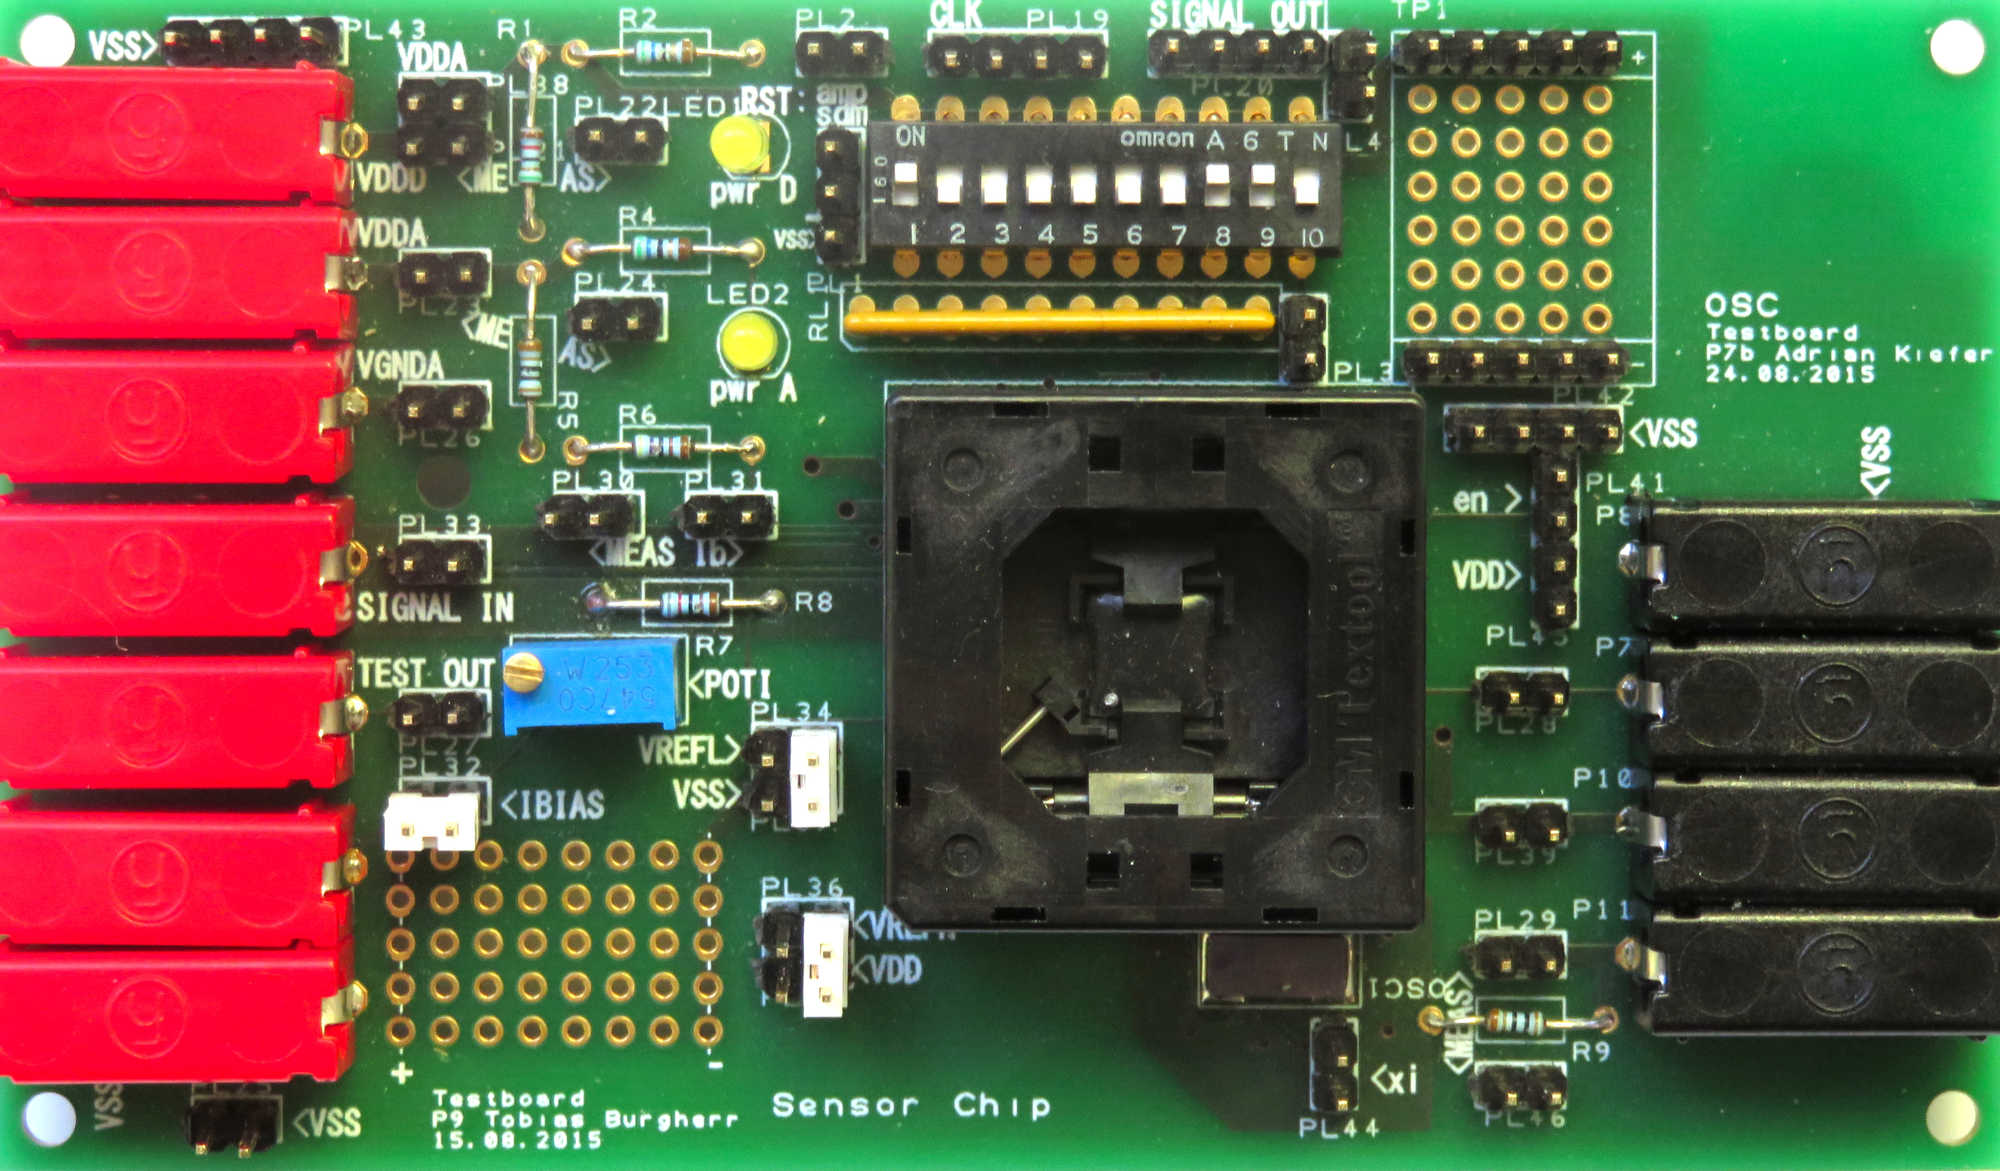
\includegraphics[width=135mm]{images/pcb/pcbOverview.jpeg}};
    \end{scope}
    %\node[fill=black,text=white,anchor=south west] at (0mm,0mm) {\textsf{\Large{VDDD}}};

    \node[%
        %fill=black,
        %fill opacity=0.5,
        text=white,
        text opacity=1,
        rounded corners=1mm,
        anchor=south west] at (4mm,66mm) {\plugtext{VDDD}};

    \node[%
        %fill=black,
        %fill opacity=0.5,
        text=white,
        text opacity=1,
        rounded corners=1mm,
        anchor=south west] at (4mm,56.5mm) {\plugtext{VDDA}};

    \node[%
        %fill=black,
        %fill opacity=0.5,
        text=white,
        text opacity=1,
        rounded corners=1mm,
        anchor=south west] at (4mm,47.5mm) {\plugtext{VGNDA}};

    \node[%
        %fill=black,
        %fill opacity=0.5,
        text=white,
        text opacity=1,
        rounded corners=1mm,
        anchor=south west] at (1mm,37.5mm) {\textbf{\textsf{\large{SIGNAL IN}}}};

    \node[%
        %fill=black,
        %fill opacity=0.5,
        text=white,
        text opacity=1,
        rounded corners=1mm,
        anchor=south west] at (1mm,27.5mm) {\textbf{\textsf{\large{TEST OUT}}}};

    \node[%
        %fill=black,
        %fill opacity=0.5,
        text=white,
        text opacity=1,
        rounded corners=1mm,
        anchor=south west] at (4mm,17mm) {\plugtext{IBIAS}};

    \node[%
        %fill=black,
        %fill opacity=0.5,
        text=white,
        text opacity=1,
        rounded corners=1mm,
        anchor=south west] at (4mm,8mm) {\plugtext{VSS}};
\end{tikzpicture}
